%% LyX 2.0.6 created this file.  For more info, see http://www.lyx.org/.
%% Do not edit unless you really know what you are doing.
\documentclass[]{paper}
\usepackage{fontspec}
 \setmainfont[Mapping=tex-text]{华文仿宋}
\setsansfont[Mapping=tex-text]{华文细黑}
\setmonofont{华文仿宋}
\usepackage{listings}
\usepackage{graphicx}
\makeatletter
\usepackage{xeCJK}

\makeatother

\usepackage{xunicode}
\usepackage{polyglossia}
\setdefaultlanguage{}
\begin{document}

\title{ 泛函分析的一些笔记}
\author{徐浩}

\maketitle
\begin{abstract}
用力学问题来求解泛函
\end{abstract}


\section{问题}
求解$\vec{x}(t)$,使得
$$\delta \int_a^b f(\vec x)dt=0$$
\subsection{解空间}
空间中的所有曲线
\subsection{解}
最优曲线

\subsection{思路}

\begin{enumerate}
\item 雪崩
\item 水流
\end{enumerate}
如何归纳这些问题的共性。
\section{张力水流}
\subsection{Assumption}
再无引力的情况下,我们认为水流会趋向于合并到表面积最小的状况。\\
符合物理原理,最小能量原理。
\subsection{定理}
合并定理\\
松弛定理
\subsection{产生方法}
随机行走\\
步长与当前f相关.\\
\subsection{合并方法}
拉链式合并
\subsection{松弛定理}
\begin{center}
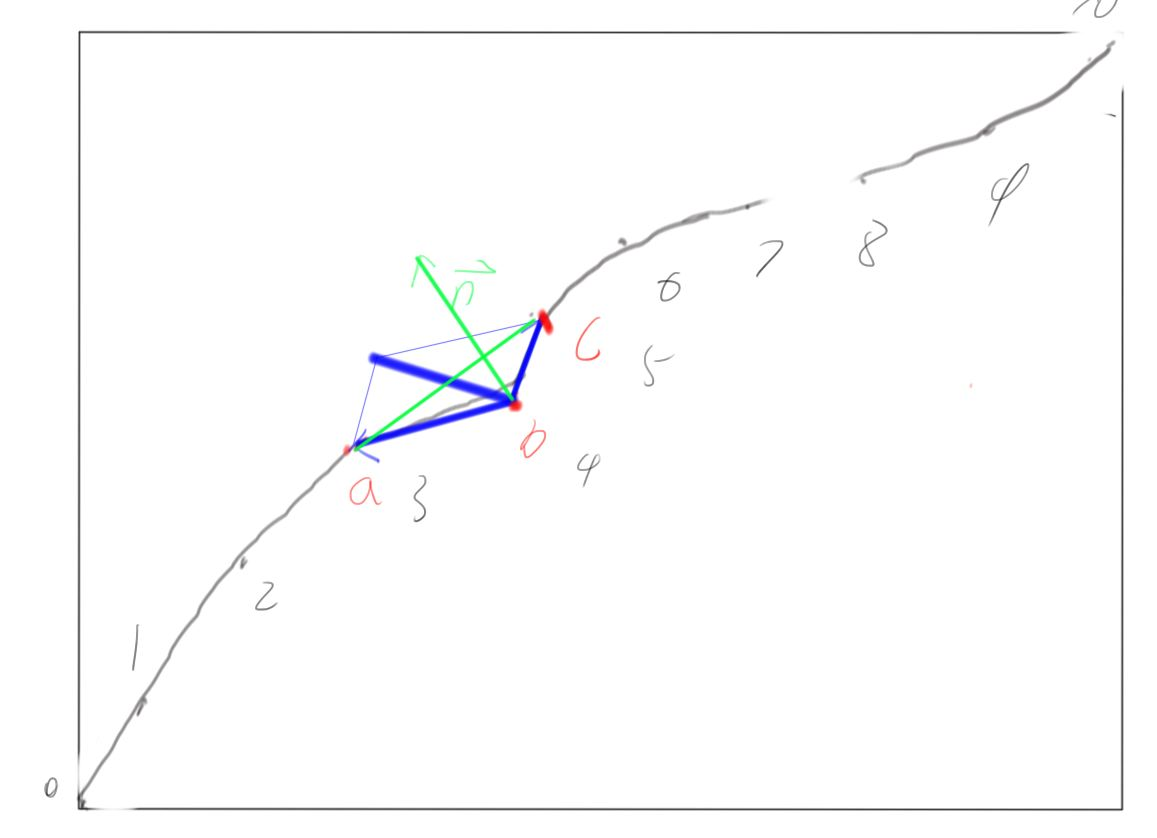
\includegraphics[width=0.7\linewidth]{./Image001}
\end{center}
那么有
\begin{eqnarray}
&&\vec{ac}=(c_x-a_x,c_y-a_y)\\
&&\vec n=(a_y-c_y,c_x-a_x)\\
&&\vec F_p=\frac{(x_i-x_{i-1},y_i-y_{i-1},z_i-z_{i-1})}{\sqrt{\Delta x^2+\Delta y^2+\Delta z^2}}\\
&&\vec F_n=\frac{(x_{i+1}-x_{i},y_{i+1}-y_{i},z_{i+1}-z_{i})}{\sqrt{\Delta x^2+\Delta y^2+\Delta z^2}}\\
&&\vec F=F_n+F_p\\
&&\vec r=\alpha\vec F\\
&&\Delta q_b=(\vec{F} \cdot \vec n)\vec{n}
\end{eqnarray}

\subsection{优点}
只用链表完成对空间中曲线的遍历
\section{雪崩或者河流的迁移}
引力牵引,合并沟槽,类似与三峡。
\section{元胞自动机?}
\end{document}
